\chapter{CPU的Verilog实现及Quartus II仿真}

\section{CPU的硬件设置}

\begin{enumerate}
\item CPU字长为8位,8个程序员可见的寄存器,分别命名为$\mathrm{r_0,\cdots,r_7}$。
\item 地址总线、数据总线各为8位,可访问$2^8$字节的地址空间。
\item 存储器由ROM和RAM组成,出于简便,系统工作区(ROM),用户工作区(RAM)分开编址。对于RAM,读操作时无需显式给出读命令,但在地址有效后需要等待一个周期才能获得数据;写操作时需要显式给出写命令(WE),且要满足地址、数据的建立与保持时间要求。
\item 采用1字节或者2字节变长指令字,操作码采用定长格式。二字长指令在取指阶段需要访问两次内存。
\item 设置指令标记寄存器,存储当前运行指令的类别。
\item 采用定长三级时序,每个指令周期包含3 个机器周期(取指周期、间址周期和执行周期),每个机器周期由3个节拍构成。用节拍(beat)控制指令的运行
\item 设置程序计数器(PC),指令寄存器(IR),存储器地址寄存器(MAR),存储器数据寄存器(MDR),累加器(ACC),寄存器地址寄存器(RADD,用来存储寄存器型指令中寄存器的地址)。
\end{enumerate}

\section{主要模块的Verilog实现}

\subsection{取指周期的指令译码操作}

\begin{lstlisting}[language=Verilog]
	case (q_w[7:5])
	3'b000:	begin//mov
			case(q_w[4:3])
			2'b00:	begin//mov reg-reg
					instruction <= 5'b00000;
					radd1 <= q_w[2:0];
					pc <= pc+1;
					jp <= 2;
					end
			2'b01:	begin//mov reg-mem;
					instruction <= 5'b00001;
					radd1 <= q_w[2:0];
					pc <= pc+1;
					jp <= 2;
					end
			2'b10:	begin//mov mem-reg;
					instruction <= 5'b00010;
					radd2 <= q_w[2:0];
					pc <= pc+1;
					jp <= 2;
					end
			2'b11:	begin//mov reg-`立即数`;
					instruction <= 5'b00011;
					radd1 <= q_w[2:0];
					pc <= pc+1;
					jp <= 2;
					end
			endcase
			end
	3'b001:	begin//add
			case(q_w[4:3])
			2'b00:	begin//add reg-reg;
					instruction <= 5'b00100;
					radd1 <= q_w[2:0];
					pc <= pc+1;
					jp <= 2;
					end
			2'b01:	begin//add reg-mem;
					instruction <= 5'b00101;
					radd1 <= q_w[2:0];
					pc <= pc+1;
					jp <= 2;
					end 
			2'b10:	begin//add reg-`立即数`;
					instruction <= 5'b00110;
					radd1 <= q_w[2:0];
					pc <= pc+1;
					jp <= 2;
					end
			endcase
			end
	3'b010: begin//sub
			case(q_w[4:3])
			2'b00:	begin//sub reg-reg;
					instruction <= 5'b01000;
					radd1 <= q_w[2:0];
					pc <= pc+1;
					jp <= 2;
					end
			2'b01:	begin//sub reg-mem;
					instruction <= 5'b01001;
					radd1 <= q_w[2:0];
					pc <= pc+1;
					jp <= 2;
					end
			2'b10:	begin//sub reg-`立即数`;
					instruction <= 5'b01010;
					radd1 <= q_w[2:0];
					pc <= pc+1;
					jp <= 2;
					end
			endcase
			end
	3'b011: begin//and
			case(q_w[4:3])
			2'b00:	begin//and reg-reg;
					instruction <= 5'b01100;
					radd1 <= q_w[2:0];
					pc <= pc+1;
					jp <= 2;
					end
			2'b01:	begin//and reg-mem;
					instruction <= 5'b01101;
					radd1 <= q_w[2:0];
					pc <= pc+1;
					jp <= 2;
					end
			2'b10:	begin//and reg-`立即数`;
					instruction <= 5'b01110;
					radd1 <= q_w[2:0];
					pc <= pc+1;
					jp <= 2;
					end
			endcase
			end
	3'b100: begin//or
			case(q_w[4:3])
			2'b00:	begin//or reg-reg;
					instruction <= 5'b10000;
					radd1 <= q_w[2:0];
					pc <= pc+1;
					jp <= 2;
					end
			2'b01:	begin//or reg-mem;
					instruction <= 5'b10001;
					radd1 <= q_w[2:0];
					pc <= pc+1;
					jp <= 2;
					end
			2'b10:	begin//or reg-`立即数`;
					instruction <= 5'b10010;
					radd1 <= q_w[2:0];
					pc <= pc+1;
					jp <= 2;
					end
			endcase
			end
	3'b101:	begin//not
			instruction <= 5'b10100;
			radd1 <= q_w[2:0];
					jp <= 2;
			end
	3'b110: begin//jmp
				instruction <= 5'b11000;
				pc <= pc + 1;
				jp <= 2;
				end
	3'b111: instruction <= 5'b11100;//hlt
	default:jp<= 2;
	endcase
\end{lstlisting}
Verilog程序较长,为避冗杂,这里不再列出。另有源码附上。
\section{Quartus II仿真与测试}
可以手动将汇编代码编译成该CPU可以识别的机器代码。由于缺少条件转移指令,无法实现循环和条件分支,这里我增加了一条jnz指令,当运算结果不为0是,程序跳转到目标代码处,跳转地址由指令直接给出。
\begin{lstlisting}[language={[x86masm]Assembler}]
mov r1,0;
mov r2,8;
for: add r1,1;
sub r2,1;
jz for;
hlt;
\end{lstlisting}
波形仿真结果在
\begin{figure}[H]
\centering
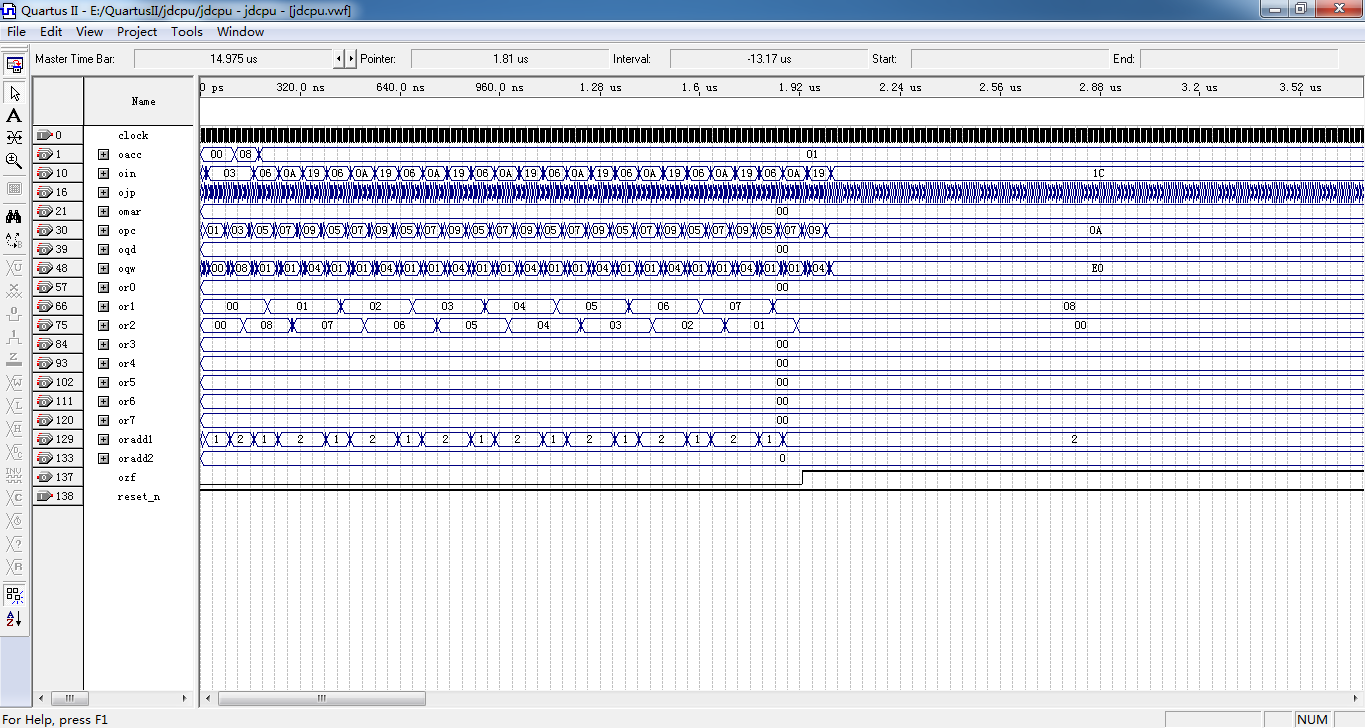
\includegraphics[scale=0.45]{vector.png}
\caption{仿真输出波形}
\end{figure}